%----------------------------------------------------------------------------
\chapter{Bevezetés}
%----------------------------------------------------------------------------
A szoftverfejlesztés terén egyre nagyobb szerepet kap a modellvezérelt tervezés. A módszer lényege, hogy a rendszert magas absztrakciós szintű modellekkel írjuk le, később ezeket folyamatosan finomítjuk, majd futtatható forráskódot generálunk belőlük, ezzel megkönnyítve és meggyorsítva a fejlesztés folyamatát. Modellek alkalmazásával komplex rendszerek is sokkal átláthatóbbá válhatnak.

Ezeken a projekteken általában egyszerre többen is dolgoznak, ami felveti a biztonság kérdéskörét is. A modellnek lehetnek olyan privát részei, amelyekhez csak bizonyos felhasználók férhetnek hozzá, kritikus pontjai, amelyeket csak a megfelelő szakértelemmel rendelkező fejlesztők módosíthatnak. A kollaborációban részt vevő fejlesztők, csapatok gyakran különböző szaktudással rendelkeznek, a rendszer más és más részeinek elkészüléséért felelősek, amihez elég, ha a modell releváns részéhez férnek csak hozzá. Azt, hogy a különböző felhasználók milyen modell elemeket írhatnak és olvashatnak, a hozzáférés-szabályozás mondja meg.

%----------------------------------------------------------------------------
\section{Hozzáférés-szabályozás lehetőségei}
%----------------------------------------------------------------------------
%----------------------------------------------------------------------------
\subsection{Fájl szintű hozzáférés-szabályozás}
%----------------------------------------------------------------------------
Fájl szintű hozzáférés szabályozás esetén, ha egy felhasználónak csak a modell egy bizonyos fragmenséhez szeretnénk jogosultságot biztosítani, akkor a modellnek ezt a részét le kell választanunk és külön kell eltárolnunk, a fájl tulajdonságai között pedig beállítani, hogy a felhasználó számára publikus legyen. Újabb felhasználók és szabályok hozzáadásával azonban egyre inkább felaprózódhat a modell, ahogy azt a lenti ábra szemlélteti. Összetettebb, több felhasználós rendszerek esetén ez megnehezíti a fejlesztés folyamatát.

\begin{figure}[!ht]
	\centering
	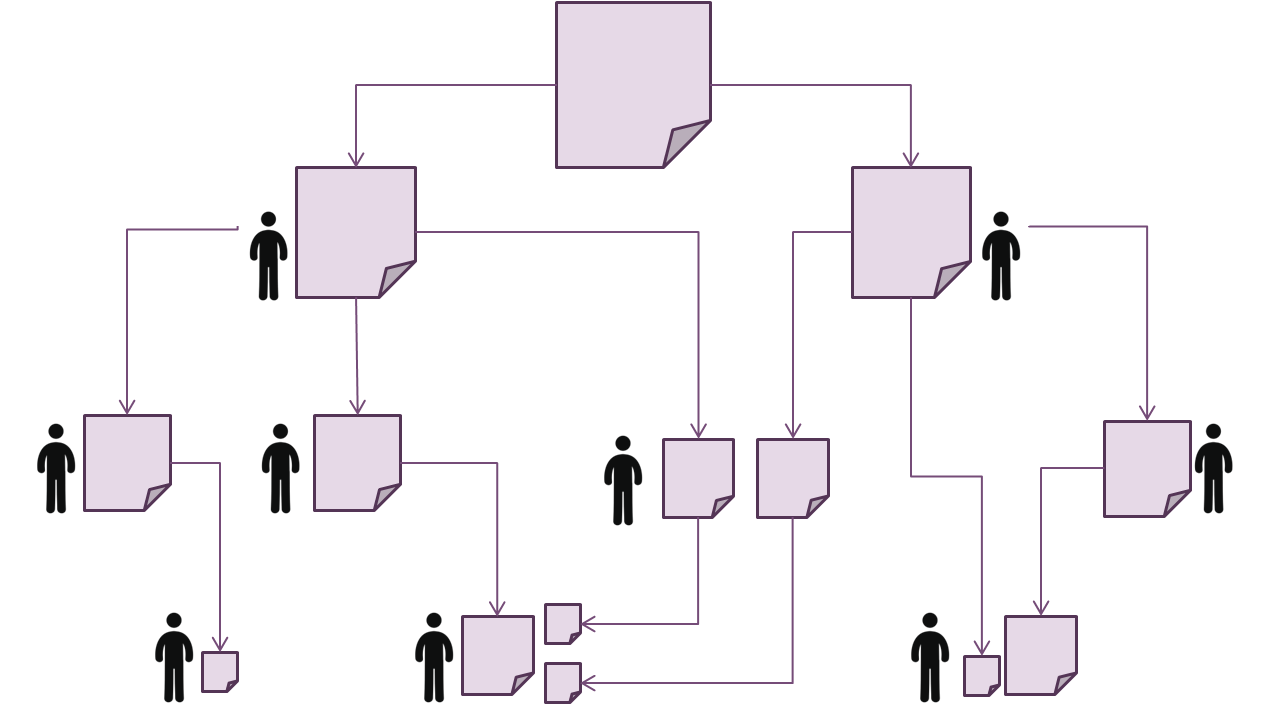
\includegraphics[width=150mm, keepaspectratio]{figures/fileLevel.png}
	\caption{A fájl szintű hozzáférés-szabályozás hátránya}
	\label{fig:fileLevel}
\end{figure}

%----------------------------------------------------------------------------
\subsection{Szabály alapú hozzáférés-szabályozás\protect\footnote{Gabor Bergmann, Csaba Debreceni, Istvan Rath, and Daniel Varro: Query-based Access Control for Secure Collaborative Modeling using Bidirectional Transformations, 2016}}
%----------------------------------------------------------------------------
Az előbbinél hatékonyabb lehet egy szabály alapú hozzáférés-szabályozás, amely során modell szinten, szabályokban fogalmazhatjuk meg, hogy ki milyen olvasási/írási jogosultsággal rendelkezzen a különböző modell elemek felett. Ezen szabályok betartásáért egy ún. lencse felel, ez egy kétirányú modell transzformáció, aminek műveletei a GET és a PUTBACK. Előbbi minden felhasználó számára egy egyedi nézetet készít a modellből, amelyen csak azok a modell elemek (objektumok, attribútumok, referenciák) szerepelnek, amiket a szabályok szerint láthat. A módosítások a PUTBACK művelettel érvényesíthetők, ami előbb ellenőrzi az írási jogosultságokat, és amennyiben azok teljesülnek, végrehajtja a változást, ha nem, akkor visszautasítja a műveletet.

\begin{figure}[!ht]
	\centering
	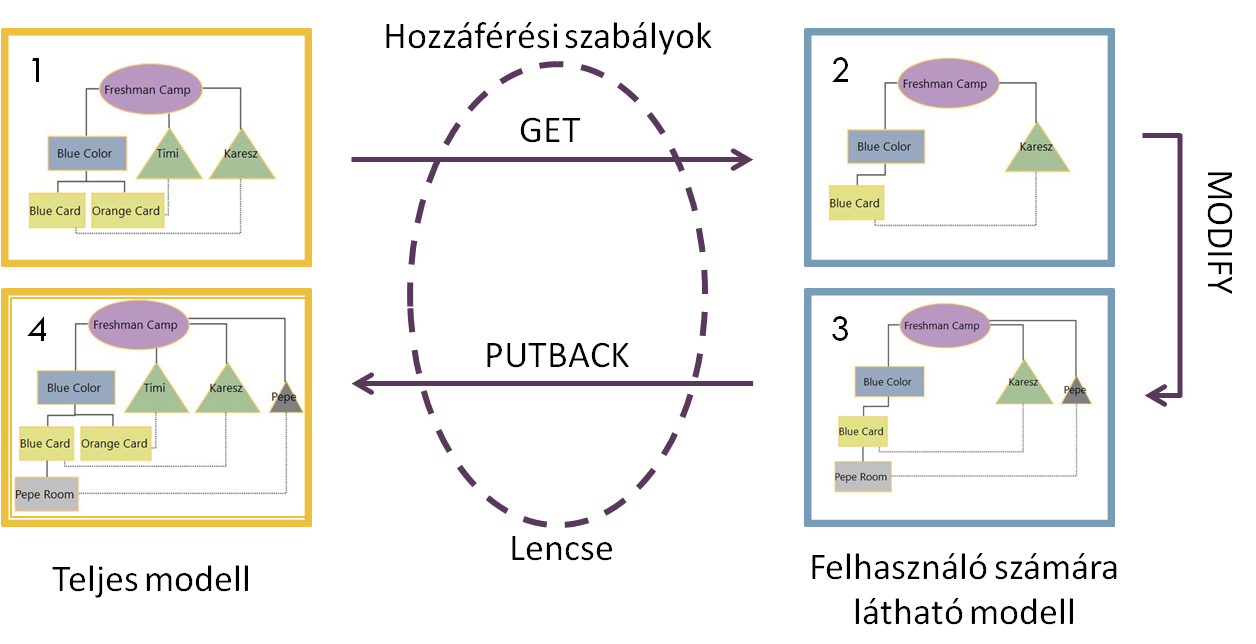
\includegraphics[width=150mm, keepaspectratio]{figures/lens.png}
	\caption{A szabályok betartásáért felelős lencse működése}
	\label{fig:lens}
\end{figure}

\clearpage
%----------------------------------------------------------------------------
\section{MONDO Collaboration Framework}
%----------------------------------------------------------------------------
A MONDO kutatási projekt keretei közt készült egy kollaborációs keretrendszer, amely a másodikként említett szabály alapú hozzáférés-szabályozást alkalmazza. Ennek hiányossága, hogy nem veszi figyelembe az alapértelmezettként megadott hozzáférési szabályokat, valamint az olvasási és írási függőségeket. Az alapértelmezett szabályokat akkor vesszük figyelembe, ha egy modell elemre nincs definiálva egyéb specifikus szabály. Olvasási vagy írási függőségről pedig például akkor beszélünk, amikor egy modell elem látható/módosítható, de az őt tartalmazó elem nem, vagy amikor egy modell elem nem látható, de módosítható. A célom egy olyan, elméletben már létező algoritmus\footnote{Csaba Debreceni, Gábor Bergmann, István Ráth and Dániel Varró: Deriving Effective Permissions for Modeling Artifacts from Fine-grained Access Control Rules, 2016} implementálása, amelynek célja, hogy ezeket a konfliktusokat feloldja.
